\scanpage{50}
% archive foliation: 49
% lines 1-8
\begin{tabular}{c}
U N I V E R S I T E\\
DES SCIENCES ET TECHNIQUES\\
DU LANGUEDOC\\
\texttt{------------}\\
Service de la Scolarité\\
MR/GJ\\
Diffusion : Liste H\\
N°3548
\end{tabular}

MONTPELLIER, le 8 JUIN 1978
% line 9
\uline{AVIS DE SOUTENANCE D'UNE THESE DE DOCTORAT D'ETAT}
% line 10
\uline{Nom et prénom de la candidate} : LINDHEIMER née MONNIER Arlette
% lines 11-12
\uline{Titre de la thèse} : Contribution à l'étude diffusiométrique des électrolytes dans des solvants mixtes de constantes diélectriques variables.
% lines 13-15
\uline{Date, heure et lieu de soutenance prévus} :

1er JUILLET 1978 à 9 Heures 30 mn

Salle de cours n° 2, U.S.T.L.
% line 16
\uline{Nom du Directeur de thèse} : Monsieur le Professeur B. BRUN
% lines 17-18
\uline{Désignation du laboratoire où la thèse est préparée} :

Laboratoire des Interactions moléculaires, U.S.T.L.
% lines 19-23
\uline{Résumé de la thèse} : Les coefficients de diffusion ioniques ont été mesurés à 25°C pour des électrolytes dissous dans des solvants mixtes dont les constantes diélec-\\
triques prenaient des valeurs différentes :

- soit élevées comme dans les mélanges eau-N-méthylpropionamide,

- soit faibles comme dans les mélanges eau-alcool et eau-éther.
% lines 24-27
Dans le premier cas, la loi étendue relative au coefficient de diffusion a été vérifiée jusqu'à 0,2M environ ; dans les autres cas la présence d'associations ioniques a été mise en évidence et les paramètres d'associations ont été obtenus dans le cadre du modèle des paires d'ions.
% line 28
\uline{Durée approximative des recherches ayant abouti à la thèse} : 5 ans
% lines 29-32
\uline{Noms des Rapporteurs} :

\begin{tabular}{ll}
SANFELD A. & Professeur, Chimie Physique, Univ. BRUXELLES\\
TURQ P. & Chargé de Cours, Chimie Physique, Univ. PARIS\\
BRUN B. & Professeur, Chimie Physique, U.S.T.L.
\end{tabular}
% lines 33-43
\uline{Composition du jury} :

\begin{tabular}{lp{.74\linewidth}}
BRUN B. & Professeur, Chimie Physique, Univ. Sciences et Techn. Languedoc\\
& MONTPELLIER\\
& (Président)\\
SANFELD A. & Professeur, Chimie Physique, Univ. BRUXELLES\\
TURQ P. & Chargé de Cours, Chimie Physique, Univ. PARIS\\
& (Membre extérieur choisi en raison de sa compétence scientifique)\\
GROMB S. & Professeur, Chimie Physique, U.S.T.L.\\
GIRAL L. & Professeur, Chimie Organique,U.S.T.L.\\
& (Membre étranger à la spécialité de la candidate)
\end{tabular}
% lines 44-46, lower right
Le Secrétaire Général,

\figure{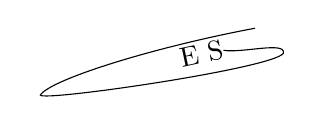
\begin{tikzpicture}[scale=.8]
\node[rotate=12] at (.55,.2) {\unsure{E S}};
\draw (1.4,.6) .. controls (-.2,.3) and (-1.8,-.2) .. (-2,-.45) .. controls (-2.2,-.6) and (1.65,-.05) .. (1.85,.2) .. controls (1.9,.4) and (1.2,.2) .. (.9,.25);
\end{tikzpicture}}

\uline{E. SIAU}
% lines 47-48, lower-left label
MR LE PROFESSEUR GROTHENDIECK A.

MATHEMATIQUES\qquad 5
